%-----------------------------------------------------------------------------%
\chapter{\babTiga}
%-----------------------------------------------------------------------------%

Pada bab ini, kita membahas model sistem yang dianalisis, dan kuantitas fisis yang dihitung. Selanjutnya, sebelum membahas pengembangan metode penyelesaian impuritas yang baru, kita terlebih dahulu membahas metode penyelesaian impuritas yang sederhana dari DMFT, yakni medan rata-rata, dan teori iterasi pertubasi, yang kita pelajari sebagai hasil pembanding dari metode penyelesaian impuritas yang kita kembangkan, yakni flutuasi okupansi.

%-----------------------------------------------------------------------------%
\section{Model Hamiltonian dan Kuantitas Fisis}
%-----------------------------------------------------------------------------%

Model Hamiltonian yang akan dipelajari dalam skripsi ini adalah hamiltonian Hubbard khusus pada kasus \textit{half-filling}, yang dimana dengan memastikan bahwa untuk setiap parameter $U$, memiliki potensial kimia $\mu = 0$, maka hamiltonian ditulis sebagai persamaan (2.56)
\begin{align}
H = \sum_{\left< i,j \right> , \sigma} -\left(t_{ij} c^\dagger_{i,\sigma}c_{j,\sigma} + h.c. \right) + U \sum_i \left( n_{i\uparrow} - \frac{1}{2}\right) \left(n_{i\downarrow} - \frac{1}{2} \right)
\end{align}
pada skripsi ini juga hanya mempertimbangkan suku kinetik hopping $t_{ij}$ hanya pada tetangga terdekat saja, sehingga hamiltonian diatas lebih dapat disederhanakan sebagai
\begin{align}
H = -t\sum_{\left< i,j \right> , \sigma} \left( c^\dagger_{i,\sigma}c_{j,\sigma} + h.c. \right) + U \sum_i \left( n_{i\uparrow} - \frac{1}{2}\right) \left(n_{i\downarrow} - \frac{1}{2} \right)
\end{align}
dimana suku hopping bernilai non-negatif $t \geq 0$. 

Fungsi Green hamiltonian Hubbard untuk hamiltonian Hubbard pada persamaan (3.2) adalah
\begin{align}
G_\sigma(z) = \frac{1}{z - \epsilon_\bo{k} - \Sigma_\sigma(z)}
\end{align}
dimana $\Sigma_\sigma(z)$ adalah kuantitas \textit{self-energy} yang berhubungan dengan suku interaksi $U$, yang diselesaikan dengan beberapa model impuritas yang akan dijelaskan dan digunakan dibawah.

\subsection{Kisi Bipartite}

Agar kita dapat menginvestigasi keadaan antiferromagnetik pada model Hubbard, maka model impuritas untuk satu kisi tidak cukup untuk bisa menghasilkan hasil \textit{magnetic order}. Cara yang paling sederhana adalah membentuk kisi bipartite dimana didalamnya terdiri dari dua \textit{sublattice} A dan B, lihat gambar 3.1, dengan dua \textit{self-energy} yang berbeda, $\Sigma^A_\sigma \neq \Sigma^B_\sigma$ \cite{sublattice}.

\begin{figure}
	\centering
	\includegraphics[width=0.80\textwidth]
		{pics/sublattice.png}
	\caption{Kiri: Gambaran skematik \textit{sublattice} AB untuk bisa memperoleh keadaan Neel. Kanan: Zona Brillouin Magnetik, daerah Zona Brillouin pertama dari keadaan Neel.}
\end{figure}

Dari skema tersebut, kita bentuk operator $a^\dagger_{i\sigma}$ dan $b^\dagger_{i\sigma}$ yang berperan sebagai operator untuk masing-masing \textit{sublattice}. Maka Hamiltonian (2.2) dapat ditulis sebagai
\begin{align}
H_0 = - t \sum_{\left< i,j \right>,\sigma} \left( a^\dagger_{i\sigma} b^\dagger_{j,\sigma} + b^\dagger_{j,\sigma}a_{i,\sigma} \right)
\end{align}
transformasi fourier ke ruang momentum $\bo{k}$ menghasilkan
\begin{align}
H_0 = \sum_\bo{k} \sum_\sigma \left( a^\dagger_{\bo{k},\sigma} b^\dagger_{\bo{k},\sigma}  \right)
\begin{pmatrix}
0 & \epsilon_\bo{k} \\
\epsilon_\bo{k} & 0
\end{pmatrix}
\begin{pmatrix}
a_{\bo{k},\sigma} \\
b_{\bo{k},\sigma}
\end{pmatrix}
\end{align}
dengan $\epsilon_\bo{k}$ adalah dispersi elektron pada model kisi. Dengan notasi ini, fungsi Green sekarang menjadi matriks dengan besar sejumlah \textit{sublattice} $n = 2$,
\begin{align}
G_{\bo{k},\sigma}(z) = 
\begin{pmatrix}
\zeta^A_\sigma & -\epsilon_\bo{k} \\
-\epsilon_\bo{k} & \zeta^B_\sigma
\end{pmatrix}^{-1}
\end{align} 
dimana $\zeta^{A/B}_\sigma = z - \Sigma^{A/B}_\sigma$. Hal ini mengimplikasikan berarti terdapat dua model impuritas efektif yang harus diselesaikan masing-masing dalam perhitungan \textit{self-consistent}. Namun, dalam keadaan Neel, terdapat penyerdehanaan yang lebih lanjut. Pada kasus ini, properti dari keadaan di basis \textit{sublattice} A dengan spin $\sigma$ memiliki properti yang samadengan basis \textit{sublattice} B dengan spin yang berlawanan $\sigma'$. Hal ini benar, terutama pada \textit{self-energy}, sehingga terdapat simetri $\zeta^A_\sigma = \zeta^B_{\sigma'} \equiv \zeta_\sigma$ yang akan tinggal kita gunakan, tanpa harus melibatkan indeks basis A dan B, melainkan hanya $\sigma \in [\uparrow, \downarrow]$.

Konsekuensinya adalah fungsi Green lokal pada model kisi, dan tetangga terdekatnya dengan indeks $i$ sekarang termasuk dalam bagian dari \textit{sublattice}. Hal ini dapat diselesaikan dengan melakukan proses inversi pada matriks dalam persamaan (3.6) dan menjumlahkan terhadap momentum $\bo{k}$, dan dalam representasi integral terhadap energi, didapat\cite{DMFT}
\begin{align}
G_{ii,\sigma}(z) = \zeta_{\sigma'} \int_{-\infty}^\infty d\epsilon \; \frac{D(\epsilon)}{\zeta_\uparrow \zeta_\downarrow - \epsilon^2}
\end{align}

\subsection{Kuantitas Fisis}

Pada skripsi ini, kuantitas fisis pertama (\textit{observable}) yang di analisis adalah DOS dari sistem elektronik model, dimana ini dapat dihitung dari hubungannya dengan fungsi Green lokal, yang ditunjukkan oleh persamaan (2.40),
\begin{align}
D(\omega) = - \frac{1}{\pi} \text{Im} [G(\omega + i0^+)]
\end{align}
Dari DOS ini kita dapat mempelajari fasa metal dan isolator dari sistem, dan transisi keduanya. Hal ini dilihat dari jumlah keadaan (\textit{spectral weight}) pada daerah energi fermi $\epsilon_f = \mu$. Dikarenakan hamiltonian Hubbard pada persamaan (3.2) yang digunakan pada skripsi ini mengakomodir $\mu =0$ untuk $U$ berapa saja, maka kita tinggal melihat \textit{spectral weight} pada energi $\omega = 0$. Ada dan tidaknya batas antar dua pita (gap) yang akan menentukan apakah sistem tersebut metal atau isolator.

Kuantitas fisis kedua yang kita analisis berikutnya adalah besar magnetik sistem. Magnetik sistem secara sederhana dihitung dari perbedaan okupansi elektron dengan spin up dan spin down. Pada kasus half-filling dalam kisi bipartite, kondisi \textit{magnetic order} yang mungkin adalah antiferomagnetik, dan juga dikarenakan simetri keadaan Neel $\Sigma^A_\sigma = \Sigma^B_{\sigma'}$, maka hasil magnetisme secara keseluruhan bernilai nol, dimana $M_A = - M_B$. Namun, pada kondisi antiferomagnetik $M_A = - M_B \neq 0$, sehingga dengan disini kita menganalisis besar perbedaan okupansi spin up dan down untuk satu \textit{sublattice}. Dengan melihat perbedaan okupansi tersebut, kita bisa mempelajari apakah sistem berada dalam keadaan antiferomagnetik atau paramagnetik ($M_A = - M_B \approx 0$). 

Okupansi sendiri dapat dihitung dari fungsi Green lokal,
\begin{align}
n_{i\sigma} = \frac{1}{\pi} \int d\omega \;  \text{Im} [G_{ii,\sigma}(\omega + i0^+)] f(\omega,T) = - \int d\omega\; D(\omega) f(\omega,T)
\end{align}
dimana $f(\omega,T)$ adalah distribusi fermi pada setiap keadaan energi $\epsilon$ dalam tempeartur $T$,
\begin{align}
f(\omega,T) = \frac{1}{\exp(\epsilon\beta) + 1}; \quad \beta = \frac{1}{k_BT}
\end{align}
distribusi fermi diperlihatkan oleh gambar 3.2.

\begin{figure}
	\centering
	\includegraphics[width=1.0\textwidth]
		{pics/fermi.pdf}
	\caption{Distribusi elektron pada setiap energi diatur oleh distribusi fermi, diperlihatkan untuk temperatur yang berbeda.}
\end{figure}

Sehingga besar perbedaan okupansi atau magnetisasi untuk satu \textit{sublattice} dihitung dengan
\begin{align}
M_i = \frac{n_{i\uparrow} - n_{i\downarrow}}{n_{i\uparrow} + n_{i\downarrow}}
\end{align}

%-----------------------------------------------------------------------------%
\section{Model Kisi}

Model kisi sederhana diperlukan diperlukan untuk menganalisis keberhasilan metode penyelesaian impuritas, sebelum menghitung lebih lanjut pada kasus material asli. Sederhana yang dimaksud adalah model kisi memiliki satu orbital saja, dan memiliki simetri yang sederhana. Model kisi sederhana ini masih mampu menangkap properti dari sistem terkorelasi kuat, sehingga hasil yang didapatkan sepenuhnya hanya bergantung pada metode penyelesaian impuritas.

\subsection{Kisi Bethe}

Kisi Bethe adalah kisi yang memiliki jumlah koordinasi $q$ tidak berhingga. Sehingga pada batas ini, hasil dari DMFT menjadi eksak. Karakteristik spesial lainnya adalah, setiap dua posisi site yang berbeda, keduanya dihubungkan dengan lintas terpendek yang unik (gambar 3.3). Pada dasarnya, kisi Bethe adalah kisi non-fisis, dikarenakan hilangnya simetri translasi invarian pada $q > 2$.

\begin{figure}
	\centering
	\includegraphics[width=0.60\textwidth]
		{pics/bethe.png}
	\caption{Gambaran skematik dari kisi Bethe dengan jumlah koordinasi $q = 4$. Kisi Bethe sendiri adalah tak berhingga jumlahnya, dan setiap site pada kisi saling ekuivalen.}
\end{figure}

Penyerdehanaan paling penting terjadi pada koordinasi tak berhingga $( q \rightarrow \infty )$, dimana \textit{self-energy} menjadi bersifat lokal pada ruang spasial, sehingga DMFT pada daerah ini menjadi eksak. Terlebih, bentuk DOS bethe lattice untuk kondisi yang tidak berinteraksi sangat sederhana, yakni semi-lingkaran. Dapat dibuktikkan DOS untuk sistem yang tidak berinteraksi (diturunkan di Lampiran 1), yakni
\begin{align}
D_{0,\text{bethe}}(\omega) = \frac{1}{2 \pi t^2} \sqrt{\omega^2 - 4t^2}
\end{align}
Bentuk DOS ini diperlihatkan oleh gambar 3.4. Kisi Bethe sangat penting sebagai kisi mainan (\textit{toy-lattice}) untuk mengklarifikasi transisi Mott-Hubbard logam-isolator pada kasus \textit{half-filling}, dan sering digunakan sebagai kisi untuk melihat hasil pengembangan metode-metode penyelesaian impuritas.

\subsection{Kisi Kubik}

Aproksimasi yang dilakukan DMFT adalah melihat \textit{self-energy} bersifat lokal, yakni tidak bergantung secara spasial pada ruang momentum $\bo{k}$. Sifat lokal berlaku pada jumlah koordinasi kisi menuju tak berhingga $q \rightarrow \infty$, namun pada jumlah koordinasi yang berhingga, pada dasarnya \textit{self-energy} tidak bersifat lokal. Sehingga penggunaan sifat lokal pada dimensi yang berhingga seperti kisi kubik, membuat DMFT sebagai metode yang menghasilkan aproksimasi saja pada kasus tersebut.

Tantangan utama implementasi pada dimensi berhingga adalah melihat seberapa akurat DMFT mengakomidir hasil yang mendekati walaupun mengabaikan korelasi spasial. Beberapa pekerjaan dengan metode penyelesaian impuritas telah dilakukan\cite{staudt,kent,rohringer,daniel} yang beberapa diantaranya sampai mengembangkan metode penyelesaian impuritas yang memasukkan korelasi spasial didalamnya, seperti \textit{Dynamic Cluster Approximation} (DCA)\cite{dca}. Sehingga kisi kubik adalah menjadi contoh menarik yang paling sederhana pada kasus dimensi berhingga.

Kisi kubik sendiri dikarenakan memiliki posisi atom tetangga terdekat $\bo{R}_j \in [(1,0,0), (0,1,0), (0,0,1)]$, sehingga energi dispersi pada kisi kubik adalah
\begin{align}
\epsilon_\bo{k} = -t \sum_j e^{-i\bo{k}\cdot\bo{R}_j} = -2t \left[ \cos(k_x) + \cos(k_y) + \cos(k_z) \right]
\end{align}
dengan jarak lattice di set $a = 1$. Sehingga DOS untuk kisi kubik pada kasus tidak berinteraksi adalah
\begin{align}
D_{0,\text{kubik}}(\omega) = \sum_\bo{k} \delta(\epsilon - \epsilon_\bo{k}) = \sum_{kx,ky,kz} \delta (\epsilon + 2t \left[ \cos(k_x) + \cos(k_y) + \cos(k_z) \right])
\end{align}
Bagusnya, DOS diatas masih bisa diturunkan secara analitik, sehingga tidak perlu melakukan perhitungan komputasi sumasih multi-dimensi dengan jumlah titik yang banyak sehingga memakan banyak sumberdaya komputasi. DOS diatas secara analitik (diturunkan pada lampiran 1), diberikan oleh\cite{anna}
\begin{align}
D_{0,\text{kubik}}(\omega) = \frac{1}{2\pi^3t}\int_{-1}^1 \frac{dz}{\sqrt{1-z^2}}K(m); \quad m = 1 - \left(\frac{\tilde{\omega} + z}{2}\right)^2
\end{align}
dengan $\tilde{\omega} = \omega / 2t$, dan $K(m)$ adalah integral spesial yang disebut sebagai integral elipitik komplit,
\begin{align}
K(m) = \int_0^{\pi/2} \frac{d\varphi}{\sqrt{1 - m\sin^2\varphi}}
\end{align}
Bentuk DOS kubik diperlihatkan pada gambar 3.4.

\begin{figure}
	\centering
	\includegraphics[width=0.80\textwidth]
		{pics/bethe-kubik.pdf}
	\caption{DOS pada sistem yang tidak berinteraksi untuk kedua model kisi sederhana, kisi bethe dan kisi kubik}	
\end{figure}


%-----------------------------------------------------------------------------%

%-----------------------------------------------------------------------------%
\section{Metode Penyelesaian Impuritas Pembanding}

\subsection{Medan Rata-Rata}
%-----------------------------------------------------------------------------%

Pendekatan medan rata-rata atau disebut juga pendekatan Hartree-Fock adalah pendekatan yang mengabaikan fluktuasi medan didalamnya\cite{mf}, yakni fluktuasi densitas elektron, yang dimana fluktuasinya didefinisikan sebagai $\Delta n_{i\sigma} \equiv n_{i\sigma} - \left< n_{i\sigma} \right>$, yakni jumlah perbedaan densitas elektron dari operator eksak $n_{i\sigma}$ dan okupansi rata-ratanya $\left< n_{i\sigma} \right>$. Dari relasi ini, didapatkan
$n_{i\sigma} \equiv \left< n_{i\sigma} \right> + \Delta n_{i\sigma}$. Maka operator interaksi elektron dalam kisi ditulis
\begin{align}
n_{i\uparrow}n_{i\downarrow} &= (\Delta n_{i\uparrow} + \left< n_{i\uparrow} \right>)\cdot (\Delta n_{i\downarrow} + \left< n_{i\downarrow} \right>)\notag\\
&= \Delta n_{i\uparrow} \Delta n_{i\downarrow} + \sum_\sigma n_{i\sigma} \left< n_{i\sigma} \right> - \left< n_{i\uparrow} \right> \left< n_{i\downarrow} \right>
\end{align}
Dalam pendekatan medan rata-rata, kita mengabaikan fluktuasi pada suku pertama, maka hamiltonian Hubbard pada persamaan 3.2 pada suku interaksi menjadi
\begin{align}
H_U^{MF} = U \sum_{i\sigma} n_{i\sigma} \left< n_{i\bar{\sigma}} \right> - UN \left< n_{\uparrow} \right> \left< n_{\downarrow} \right> - \frac{U}{2} \sum_{i\sigma} n_{i\sigma} + \frac{U}{4}
\end{align}
dimana $N$ adalah jumlah elektron, dan pada \textit{half-filling} ini bernilai $1$. Kondisi ini akan memastikan bahwa $\mu = 0$. Pada paramagnetik, $\left< n_{i\bar{\sigma}} \right> = \frac{1}{2}$, sehingga suku kedua dan keempat saling menghilangkan, sehingga tersisa
\begin{align}
H_U^{MF} = U \sum_{i\sigma} n_{i\sigma} \left< n_{i\bar{\sigma}} \right> - \frac{U}{2} \sum_{i\sigma} n_{i\sigma}
\end{align}

Suku interaksi sekarang memiliki operator yang sama dengan suku kinetik \textit{hopping}, sehingga dengan transformasi fourier, hamiltonian untuk spin $\sigma$ menjadi matriks 2x2 dengan 
\begin{align}
\begin{pmatrix}
U\left< n_{1\bar{\sigma}} \right> & \epsilon_\bo{k}\\
\epsilon_\bo{k} & U\left< n_{2\bar{\sigma}} \right>
\end{pmatrix}
\end{align}
ini dapat dengan mudah dilakukan diagonalisasi baik secara analitik maupun numerik, sehingga didapat hasil fungsi Green untuk masing-masing komponen 
\begin{align}
G_{i\sigma}(\zeta) = \frac{1}{\zeta - \epsilon'_{\bo{k},\sigma}}
\end{align}
dimana $\epsilon'_{\bo{k},\sigma}$ adalah nilai eigen untuk masing-masing komponen $<i\sigma>$ pada matriks 3.20.

Perhitungan \textit{self-consistent} dilakukan pertama-tama dengan menebak okupansi untuk parameter $<U,t>$, yang akan dimasukkan pada matriks (3.20). Selanjutnya menghitung fungsi Green lokal pada persamaan (3.21), dan kemudian menghitung okupansi elektron yang diberikan pada persamaan (3.9). Konvergensi tercapai jika jumlah perbedaan hasil okupansi tebakan dan hitungan kurang dari nilai toleransi yang diberikan.

%-----------------------------------------------------------------------------%
\subsection{Teori Iterasi Pertubasi (IPT)}
%-----------------------------------------------------------------------------%

Teori iterasi pertubasi (IPT) adalah metode penyelesaian impuritas sederhana yang lebih akurat dibanding medan rata-rata. IPT melibatkan diagram feynman orde kedua\cite{DMFT}. Dapat dikatakan IPT adalah koreksi diagram pada medan rata-rata karena melibatkan hingga orde kedua, yang dimana medan rata-rata hanya sampai pada orde pertama, yakni diagram hartree. Diagram feynman untuk IPT digambarkan pada 3.5. \textit{Self-energy} dari gambar diagram feynman tersebut adalah
\begin{align}
\Sigma_{i\sigma}(i\omega_n) = U\left< n_{i\bar{\sigma}} \right> - \frac{U^2}{\beta^2} \sum_{m,p} \mathcal{G}_{i\sigma}(i\omega + i\nu_m)\mathcal{G}_{i\bar{\sigma}}(i\omega_p + i\nu_m)\mathcal{G}_{i\bar{\sigma}}(i\omega_p)
\end{align}

\begin{figure}
	\centering
	\includegraphics[width=0.50\textwidth]
		{pics/ipt.png}
	\caption{Diagram feynman orde kedua dari suku pertubasi dalam pendekatan IPT.}
\end{figure}

Perhitungan pada pekerjaan skripsi ini dilakukan pada sumbu riil, sehingga dibutunkan \textit{analytical continuation} untuk \textit{self-energy} di domain matsubara ke domain riil. Hal ini dapat kita lakukan secara analitik dengan melihat relasi dari DOS dan fungsi Green matsubara
\begin{align}
G(i\omega_n) = \int d\omega \; \frac{D(\omega)}{i\omega_n - \omega}
\end{align}
Penurunan analitik \textit{analytical continuation} bagian ini diturunkan pada Lampiran B, dimana didapat \textit{self-energy} pada domain riil sebagai
\begin{align}
\Sigma(\omega) = U\left< n_{i\bar{\sigma}} \right> - U^2 \int d\nu \int d\nu' \int d\nu'' \frac{[D^-(\nu)D^+(\nu')D^-(\nu'') + D^+(\nu)D^-(\nu')D^+(\nu'')]}{\omega + i0^+ - \nu + \nu' - \nu''}\notag
\end{align}
dimana notasi $D^+$ dan $D^-$, adalah
\begin{align}
D^+(\omega) &= f(\omega)D(\omega)\\
D^-(\omega) &= f(1 - \omega)D(\omega)
\end{align}
Dengan mengambil nilai imajinernya, dan mengintegrasi terhadap $\nu''$, didapat
\begin{align}
\text{Im}\Sigma(\omega) = -\pi U^2 \int d\nu \int d\nu' [D^-(\nu)D^+(\nu')D^-(\omega - \nu + \nu') + D^+(\nu)D^-(\nu')D^+(\omega - \nu + \nu')]
\end{align}
dimana nilai riil dari $\text{Re}\Sigma(\omega)$ didapat dari relasi kramers-kronig, yang hal ini dapat digunakan untuk fungsi kasual.
\begin{align}
\text{Re}\Sigma(\omega) = \frac{1}{\pi}\mathcal{P}\int_{-\infty}^\infty d\omega' \;\frac{\text{Im}\Sigma(\omega)}{\omega' - \omega}
\end{align}

%-----------------------------------------------------------------------------%
\section{Fluktuasi Okupansi}
%-----------------------------------------------------------------------------%

Perhitungan dengan medan rata-rata atau pendekatan Hartree-Fock, merupakan pendekatan yang menghilangkan fluktuasi okupansi didalamnya. Melalui modifikasi medan rata-rata, kami membuat model impuritas yang baru dengan memasukkan suku fluktuasi. Suku fluktuasi ini tidak sepenuhnya perhitungan yang dilakukan secara kuantum, melain suatu kuantitas semi-klasik dengan konsep yang sama seperti perhitungan medan rata-rata untuk kopel elektron-fonon\cite{el-ph} dan interaksi magnetik Hund\cite{hund}. Konsep ide ini dimulai dengan memodifikasi suku interaksi pada pada model Hubbard menjadi
\begin{align}
U \sum_i n_{i\uparrow} n _{i\downarrow} &= \frac{U}{2} \sum_i \left( n_{i\uparrow} n _{i\downarrow} + n_{i\uparrow} n _{i\downarrow} \right)\notag\\
&= \frac{U}{2} \sum_i \left[ n_{i\uparrow} \left(\left< n _{i\downarrow} \right> + \delta_{i\downarrow} \right) + n _{i\downarrow} \left( \left< n_{i\uparrow} \right> + \delta_{i\uparrow} \right) \right]
\end{align}

dimana $\delta_{i\sigma}$ adalah fluktuasi okupansi elektron. Fluktuasi ini kita jadikan sebagai kuantitas kontinu klasik yang bervariasi dari nilai minimum okupansi ($n_{min} = -1$) hingga nilai maksimumnya ($n_{max} = 1$). Perhitungan ini pertama-tama dilakukan di domain matsubara. Hal ini dikarenakan pada domain matsubara kita dapat menghitung pemberat atau probabilitas masing-masing fluktuasi okupansi. Pertama-tama, \textit{self-energy} lokal dinyatakan dalam
\begin{align}
\Sigma_{\text{loc},\sigma} = \frac{U}{2}\left(\left< n_\sigma \right> + \delta_\sigma\right) 
\end{align}
dari sini, selanjutnya kita mengkonstruksi fungsi Green lokal interaksi $\tilde{G}(i\omega_n, \delta_{\uparrow}, \delta_{\downarrow})$ yang memuat suku fluktuasi didalamnya
\begin{align}
\tilde{G}(i\omega_n, \delta_{\uparrow}, \delta_{\downarrow}) = \left[ \mathcal{G}^{-1}(i\omega_n) - \Sigma_{\text{loc},\sigma}^{-1} \right]^{-1}
\end{align}
Dari sini, aksi efektif dapat dibuat untuk fluktuasi okupansi
\begin{align}
S_{\text{eff}}(\delta_\uparrow,\delta_\downarrow) = - \sum_n \ln \det \left[ \mathcal{G}^{-1}(i\omega_n) \tilde{G}(i\omega_n,\delta_\uparrow,\delta_\downarrow) \right] e^{i\omega_n 0^+}
\end{align}
dan probabilitas didapat
\begin{align}
P(\delta_\uparrow, \delta_\downarrow) = \frac{1}{Z} \exp(-S_{\text{eff}}(\delta_\uparrow,\delta_\downarrow))
\end{align}
dengan fungsi partisi $Z$
\begin{align}
Z = \int d\delta_\uparrow \int d\delta_\downarrow \; P(\delta_\uparrow, \delta_\downarrow)
\end{align}
Sehingga dari sini kita rata-rata fungsi Green akibat dari fluktuasi
\begin{align}
G_{\text{ave}}(i\omega_n) = \int d\delta_\uparrow \int d\delta_\downarrow \; P(\delta_\uparrow, \delta_\downarrow) \tilde{G}(i\omega_n, \delta_{\uparrow}, \delta_{\downarrow})
\end{align}
maka \textit{self-energy} dihitung kembali dari persamaan Dyson dengan menggunakan fungsi Green yang telah didapat rata-ratanya akibat fluktuasi
\begin{align}
\Sigma(i\omega_n) = \left[\mathcal{G}^{-1}(i\omega_n) - G_{\text{ave}}(i\omega_n)\right]^{-1}
\end{align}
Perhitungan ini dari persamaan (3.29) hingga (3.35) adalah perhitungan \textit{self-consistent} pada domain matsubara. Namun, sebelum melanjutkan perhitungan untuk iterasi selanjutnya pada domain matsubara, perhitungan yang sama dilkaukan pada domain riil, tanpa melakukan kembali perhitungan (3.31) hingga (3.33), yang dimana kuantitasnya didapat dari perhitungan pada domain matsubara. Terakhir, dilakukan perhitungan DOS dan okupansi elektron pada domain riil, dan kembali melanjutkan ke iterasi pada domain matsubara.

Fluktuasi okupansi akan digunakan sebagai metode penyelesaian impuritas alternatif untuk mencari keadaan okupansi atau magnetisme yang lebih tepat. Sehingga akan metode fluktuasi okupansi ini akan dievaluasi dengan melihat bagaimana perbedaan relatifnya terhadap metode penyelesaian impuritas medan rata-rata biasa dan IPT. Fluktuasi okupansi akan juga coba digunakan sebagai metode koreksi dari IPT, untuk melihat apakah fluktuasi okupansi dapat memperbaiki hasil menjadi lebih baik terhadap hasil-hasil literatur yang menggunakan metode penyelesaian impuritas yang lebih eksak seperti teknik QMC.

%-----------------------------------------------------------------------------%
\section{Imlplementasi Numerik}

Berikut akan dijelaskan bagaimana detail skematik dan implementasi metode penyelesaian DMFT dalam numerik.

\subsection{Diagram Proses Perhitungan Numerik}

\begin{figure}
	\centering
	\includegraphics[width=0.90\textwidth]
		{pics/general_workflow.pdf}
		\caption{Skema umum pekerjaan numerik dari skripsi ini.}
\end{figure}

\begin{figure}
	\centering
	\includegraphics[width=0.80\textwidth]
		{pics/detail_progressblock1.pdf}
		\caption{Detail blok diagram dari implementasi algoritma teori medan rata-rata dan iterasi pertubasi teori.}
\end{figure}	

\begin{figure}
	\centering
	\includegraphics[width=0.90\textwidth]
		{pics/detail_progressblock2.pdf}
		\caption{Detail blok diagram dari implementasi algoritma okupansi fluktuasi murni }
\end{figure}	

\begin{figure}
	\centering
	\includegraphics[angle=90,origin=c,width=0.750\textwidth]
		{pics/detail_progressblock3.pdf}
		\caption{Detail blok diagram dari implementasi algoritma okupansi fluktuasi sebagai koreksi dari iterasi pertubasi teori.}
\end{figure}	

%-----------------------------------------------------------------------------%

